\chapter{Introducción} \label{cap:intro}

El objetivo de este documento es presentar JAMS, una nueva aplicación realizada como Trabajo de Fin de Grado
del Grado en Ingeniería de Computadores de la Universidad Rey Juan Carlos.


\section{La arquitectura \textit{MIPS}}\label{sec:la-arquitectura-mips}

Se les conoce con el nombre de \textbf{procesadores \textit{MIPS}} a una familia de microprocesadores que implementan
la arquitectura \textit{RISC} del mismo nombre.
Aunque esta arquitectura no ha tenido un gran éxito en los computadores personales, sí ha gozado de fama en
sistemas embebidos, enrutadores y videoconsolas como la \textit{Nintendo 64} o la \textit{PlayStation 2}. \\

\noindent Su simple diseño y baja curva de aprendizaje hace a esta arquitectura ideal para introducir a los alumnos
a los lenguajes ensamblador.


\section{\textit{IDEs}: entornos de desarrollo integrados}\label{sec:ides-entornos-de-desarrollo-integrados}

Un \textbf{entorno de desarrollo integrado} (\textit{IDE, Integrated Development Environment}) es una aplicación
informática con diversas herramientas usados en el desarrollo, construcción y depuración de \textit{software}.
Un \textit{IDE} suele estar desarrollado con dos objetivos claves en mente: maximizar la productividad del
desarrollador y evitar que este tenga que utilizar herramientas externas en su trabajo.

\noindent Existe una gran variedad de entornos de desarrollos en el mercado.
Estos se pueden clasificar de diferentes maneras.

\noindent \textbf{Según su propósito:}
\begin{itemize}
    \item \textbf{Entornos de desarrollo específicos:} son entornos pensados en el desarrollo en una
    tecnología concreta.
    Algunos ejemplos son \textit{NetBeans}, \textit{CLion} o \textit{Android Studio}.
    \item \textbf{Entornos de desarrollo generales:} son entornos que no se centran en una tecnología en concreto.
    Algunos ejemplos son \textit{Intellij IDEA}, \textit{Eclipse} o \textit{Visual Studio}
\end{itemize}

\noindent \textbf{Según su complejidad:}
\begin{itemize}
    \item \textbf{Entornos de desarrollo complejos:} son aplicaciones pesadas con una gran cantidad de
    características y funcionalidades.
    Algunos ejemplos son \textit{Intellij IDEA},
    \textit{Visual Studio} o \textit{Eclipse}.
    \item \textbf{Entornos de desarrollo ligeros:} son aplicaciones que ocupan muy poco espacio, donde
    las características más avanzadas suelen ser componentes descargables.
    Algunos ejemplos son \textit{Visual Studio Code}, \textit{Atom} o \textit{Notepad++}.
\end{itemize}


\section{Motivación}\label{sec:motivacion}

Actualmente existen varias herramientas para el desarrollo y ejecución de programas basados en
la arquitectura \textit{MIPS}.
La herramienta más famosa es el editor, ensamblador y simulador \textit{MARS}\cite{MARS}, desarrollada en
el año 2006 usando la biblioteca gráfica \textit{Swing}
\footnote{\url{https://docs.oracle.com/javase/8/docs/technotes/guides/swing/}}
y el lenguaje de programación \textit{Java}.
Otra herramienta conocida es el simulador \textit{EduMIPS64}\cite{EDUMIPS64}, desarrollada en 2014 con
la misma tecnología.

\noindent Estas dos aplicaciones presentan una serie de problemas importantes:
\begin{itemize}
    \item \textbf{Falta de herramientas:} los entornos de desarrollo \textit{MIPS} sufren de una
    carencia grave de herramientas importantes.
    Este problema afecta principalmente a \textit{EduMIPS64}, donde no existe un editor de texto y
    el ensamblador es una aplicación separada que require la línea de comandos para funcionar.
    \item \textbf{Falta de estructura de proyecto:} ninguna aplicación actual presenta una estructura
    de proyecto, indispensable para el desarrollo de aplicaciones medianas y grandes.
    \item \textbf{Falta de personalización:} al ser aplicaciones muy sencillas, ninguna permite
    personalizar la apariencia de la interfaz.
    \item \textbf{Obsolescencia:} las aplicaciones están desarrolladas con tecnologías antiguas,
    con interfaces similares a las de los programas de principio de siglo.
    \item \textbf{Falta de capacidad de expansión:} el problema más grave que presentan estas aplicaciones
    es la nula capacidad de expansión de sus características, impidiendo que otros desarrolladores
    añadan nuevas funcionalidades de manera sencilla.
\end{itemize}


\section{Objetivos}\label{sec:objetivos}

El objetivo principal de este proyecto es el desarrollo de \textbf{\textit{JAMS}
(\textit{Just Another MIPS Simulator})}, un \textbf{entorno de desarrollo integrado ligero, expandible y moderno}
centrado en los lenguajes ensamblador y, más concretamente, en el lenguaje ensamblador \textit{MIPS}.

\noindent Específicamente, en este documento se detallarán los siguientes objetivos:
\begin{itemize}
    \item Investigación sobre las tecnologías más adecuadas para el desarrollo de la aplicación.
    \item Creación de un entorno base y un \textit{framework} que permita implementar diferentes herramientas.
    \item Desarrollo de un editor, ensamblador y simulador para la arquitectura \textit{MIPS32}.
    \item Desarrollo de múltiples herramientas que permitan un desarrollo y depuración sencillos.
\end{itemize}

\noindent La aplicación deberá cumplir los siguientes requisitos:
\begin{itemize}
    \item El entorno de desarrollo debe ser moderno, cómodo, fácil de usar y enfocado en el aprendizaje.
    \item El simulador debe ser capaz de ejecutar la mayoría de programas escritos en ensamblador \textit{MIPS32}.
    \item La aplicación debe tener un sistema completo de personalización, permitiendo al usuario cambiar su apariencia.
    \item La aplicación debe ser expansible mediante el uso de complementos (\textit{plugins}).
\end{itemize}

\noindent Por último, el desarrollo de la aplicación no tiene como objetivo los siguientes puntos:
\begin{itemize}
    \item Crear un entorno de desarrollo complejo con soporte para una gran variedad de lenguajes de programación.
    \item Crear un entorno de desarrollo que permita crear código válido para entornos \textit{MIPS} reales.
\end{itemize}

\section{Metodología}\label{sec:metodologia}

Debido a que la aplicación está dividida entres secciones (base, interfaz y componentes \textit{MIPS}),
es muy importante marcar una metodología que permita un desarrollo consistente, eficiente y rápido.
A nivel de desarrollo se ha optado por una metodología ágil, con \textit{sprints} de varios meses
donde se desarrollan una serie de características claves.
Todas las características se someten a varias iteraciones donde se modifican y mejoran hasta lograr un
buen resultado.

\noindent En la base y en los componentes \textit{MIPS} también se ha seguido un
desarrollo basado en pruebas unitarias, permitiendo mantener la calidad del código mientras la
aplicación va evolucionando.

\noindent Toda la metodología ha sido implementada mediante las herramientas proporcionadas por \textit{GitHub}.
Los estados de las características asignadas a un \textit{sprint} son documentados mediante proyectos.
Las acciones obligan que las pruebas unitarias deban superarse sin errores si se desea añadir un nueva
característica a la rama principal.
Estas acciones también se emplean para generar los binarios cuando un \textit{sprint} es superado y una
nueva versión de \textit{JAMS} es lanzada.

\begin{figure}[H]
    \centering
    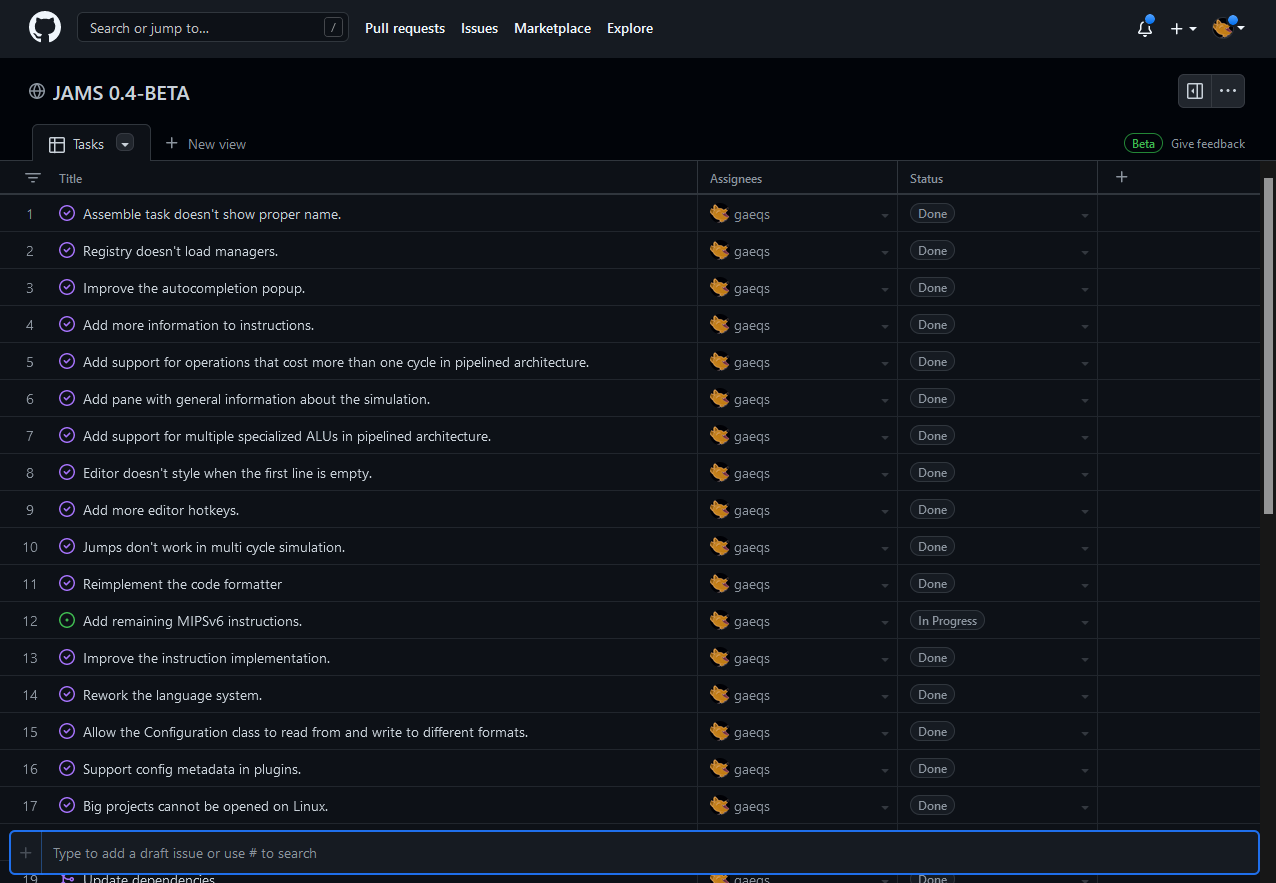
\includegraphics[width=\textwidth]{images/introduction/github}
    \caption{Proyecto de \textit{GitHub} para la versión 0.4-BETA}
    \label{fig:introduccion-github}
\end{figure}